\section{Smerte}
\textit{I dette afsnit beskrives de anatomiske og fysiologiske egenskaber ved smerte, herunder de forskellige kategorier af smerte.}

\subsection{Anatomi og fysiologi}
Smerte er af The International Association for the Study of Pain (IASP) defineret som: “\textit{An unpleasant sensory and emotional experience associated with actual or potential tissue damage, or described in terms of such damage.}” \citep{Carmon}.\\
Selvom smerte er en følelse, der forsøges undgået, er det en nødvendig mekanisme for menneskets overlevelse. Det informerer kroppen om farer eller skader som skal reageres på, så yderligere skade kan undgås.
Smerten opstår når hjernen den modtager stimuli fra neuroner i kroppen. Oplevelsen af smerte kaldes perception af smerte og er forskellig fra sensationen af smerte. Sensationen sker, når nociceptorer stimuleres og genererer et aktionspotentiale. Perceptionen sker først, når impulsen når til hjernen og smerten registreres. \citep{Martini2012}

Smerte registreres af nociceptorer som befinder sig næsten overalt i kroppen. Disse nociceptorer er frie neuronender, som forgrener sig ud i hele kroppen og ligger frit i vævet. De dækker således et stort område og kan reagere på de forskellige typer stimuli som vævet udsættes for. Nociceptorerne aktiveres af enten tryk-, stræk-, termiske og kemiske stimuli. Nociceptorerne kan også være polymodale, hvilket betyder, de kan aktiveres af flere typer stimuli. Aktiveringen af nociceptorerne sker oftest ikke direkte, men ved hjælp af transducerproteiner. Nociceptorerne kan  også aktiveres direkte, for eksempel af stofferne bradykinin og prostaglandin, som er involveret i inflammatioriske reatkioner. \citep{smerter} 
Når en nociceptor aktiveres, vil denne videre aktivere det første afferente neuron. Dette gøres ved at ionkanalerne i neuronets membran lader $Na^{2+}$ og $Ca^{2+}$ strømme ind, hvorved et gradientpotentiale opbygges. Hvis dette er tilstrækkelig højt, overskrides neuronets tærskelværdi, hvorefter et aktionspotentiale sendes afsted. Neuronfibrene, der kan lede signalet, er enten A-fibre eller C-fibre. Disse adskiller sig ved at A-fibrene er myeliniserede, hvilket C-fibrene ikke er. Dermed har A-fibre en højere ledningshastighed end C-fibre, og forårsager således den første stikkende smerte efter en vævsskade, hvorimod C-fibres aktivering forårsager en brændende smerte, der fremkommer efterfølgende. \citep{smerter} \\
Flertallet af primære afferente fibre føres til rygmarvens baghorn, hvor de danner synapse med ascenderende neuroner i rygmarven. Signaloverførslen over den første synapsekløft sker overvejende ved at de excitatoriske transmitterstoffer glutamat og substans P. 
Neuronerne viderefører signalet op gennem tractus spinothalamicus, tractus spinomesencephalicusm og tractus spinoreticularis til hjernestammen og thalamus. Thalamus er involveret i koordinering af signaler til højere strukturer, herunder det primære og sekundære sensoriske cortex, den primære motoriske cortex og det frontale cortex. Disse områder varetager blandt andet information om lokation, intensitet, adfærdsforandringer og kognitiv bearbejdning. 
Fra hjernestammen er der forbindelse til den periakvæduktale grå substans og til den rostro-ventrale medulla, som er involveret i smerteregulering via descenderende neuronfibre, som danner synapser i baghornet. I de descenderende baner er noradrenalin og serotonin de primære transmitterstoffer. \citep{smerter}

Til smertebehandling benyttes blandt andet serotonin-plus-noradrenalin-genoptagelseshæmmere (SNRI). Disse stoffer påvirker den præsynaptiske genoptagelse af serotin og noradrenalin, hvilket resulterer i en øget mængde af disse i synapsekløften, som yderligere resulterer i en øget aktivitet. Den øgede aktivitet medfører en mindsket oplevelse af smerten. \citep{smerter}

\subsection{Smertetyper}
Der findes flere måder at inddele smerte på, men generelt kan der skældnes mellem akut og kronisk smerte. \\
Hver kategori har flere undergrupperinger, som kan placeres på flere forskellige måder. \citep{Giangregorio1997} På figur \ref{smertediagram} er en oversigt over, hvordan smerte kategoriseres i dette projekt.

\begin{figure}[H]
	\centering
	\includegraphics[scale=.8]{figures/bProblemanalyse/smertediagram}
	\caption{Figuren viser hvordan smerte kan opdeles i en akut og kronisk del. Akut smerte opdeles videre i en organisk del, herunder neuropatisk og nociceptisk smerte. Kronisk smerte opdeles i både en organisk og psykogen del.}
	\label{smertediagram}
	\flushleft
\end{figure}

\subsubsection{Akut smerte}
Begræbet akut smerte dækker over den tidligere beskrevne nødvendige mekanisme, som fortæller hjernen om øjeblikkelig vævsskade, så denne hurtigt kan afværges. Akut smerte forårsages af traumer i eller på kroppen, og der skelnes mellem to typer af smerte: nociceptisk og neuropatisk. Nociceptisk smerte udløses af skade på væv herunder indre organer, overflader af kroppen og knogler. Denne type smerte skyldes aktivering af nociceptorer, som oftest sidder som frie neuronender i væv. Da nociceptorer både er inde i og uden på kroppen, opdeles nociceptisk smerte i somatisk og visceral smertesensation. Somatisk smertesensation er information fra kroppens ydre lag. Det er således sensation fra hud og muskulaturer i overfladen af torso, hoved, hals og lemmer. \citep{Martini2012} Smerten er øjeblikkelig og let placerbar. \\
Visceral smertesensation er information fra de indre organer i hals og abdomen. Sensation herfra opfattes sjældent, da de fleste indtryk er unødvendige at tage stilling til. Hvis der imidlertid opstår smerter i disse områder er denne besværlig at placere. Smerten er typisk ikke øjeblikkelig, men mere trykkende og langvarig; mavesmerter er et eksempel på visceral smerte. \citep{Martini2012} \\
Fordi viscerale og somatiske neuroner deles om samme rygmarvssegment, kan visceral information fra indre organer blive opfattet som somatisk information ved refereret smerte. Smerte på grund af skade i indre organer vil derfor typisk opfattes som somatiske smerter. Ved refereret smerte kan smerte i venstre arm og skulder således være forårsaget af smerte i hjertet. \citep{Martini2012} Nociceptisk smerte er oftest ikke årsag til kroniske smerter, med mindre smerterne bliver ved.\\ 

Neuropatisk smerte opstår af skader på nervesystemet selv, herunder neuroner, rygmarv, neurale plexi eller hjernen. 
Ved neuropatisk smerte registrer neuronerne et stimuli, som kan skyldes infektioner og sygdomme, herunder iskæmi, sclerose, diabetes og kræft. Stimuli kan ligeledes være forårsaget af smerter fra traume som startede med at være nociceptiske. Lokaliseringen af de stimulerede neuroner bestemmer hvilken form for neuropatisk smerte der percepteres. Smerten kan opleves som konstant og langvarig, hvor et typisk eksempel er fantomsmerter, men kan også være lejlighedsvis som ved hyperalgesi, hvor almindelig berøring opfattes som smertefuldt. \citep{Giangregorio1997} \citep{Carmon}

\subsubsection{Kronisk smerte}
Modsat akut smerte er kronisk smerte en længerevarende oplevelse af smerte. Kronisk smerte er af IASP defineret som smerteperception, der varer længere, end det generelt ville forventes \citep{Carmon}. Oftest sættes denne grænse ved tre måneder, men i nogle kliniske undersøgelser, eller hos nogle kræftpatienter kan smerten allerede efter en måned kategoriseres som værende kronisk. Som det kan ses af \figref{smertediagram} kan organisk smerte være både akut og kronisk. Dette sker, da kronisk smerte ofte opstår på baggrund af en akut smerte, som ikke stopper. Kronisk smerte kan således opleves af en person som enten har haft nociceptisk eller neuropatisk smerte. Kronisk smerte kan ligeledes være af psykogen oprindelse.\\
Psykogen smerte er, til forskel fra nociceptisk og neuropatisk smerte, ikke en egentlig skade på kroppens væv. Det er en imaginær perception af smerte, og derved den mest komplekse type smerte at præcisere, idet der ikke er, og muligvis aldrig har været, en fysisk årsag til smerten. Hos en person med psykogene smerter opfatter hjernen, at der forekommer nociceptiske eller neuropatiske smerter. Smerten er udelukkende psykisk hos personen, men er af den grund ikke mindre virkelig, grundet smertes subjektive natur. \citep{Giangregorio1997}

\subsection{Smerte og knæartrose}
Ledkaplser, sener, periost og spongiøst væv er tæt innerveret af nociceptorer, hvorimod ledbrusk ikke er inneveret af nociceptorer. Dette kan forklare, hvorfor  røntgenfund og smerteintensitet korrelerer i ringe grad. \citep{Petersen2016}  \citep{smerter}
Ved inflammation i ledkapslen ses en rekruttering af inaktive A- og C-fibre, hvilket kan føre til en sensibilisering af nervesystemet omkring det inflammerede område \citep{smerter}. En forlænget inflammationstid, skade på den subkondrale knogle eller en forlænget excitation af nociceptorer kan alle medføre en perifær sensibilisering, som efterfølgende kan føre til en central sensibilisering \citep{Petersen2016}.
Ved perifær sensibilisering forstås en reduktion i tærskelværdien og en øget respons af nociceptoren. Dette kan fremkomme som et resultat af vedvarende påvirkninger fra inflammitoriske mediatorer, som findes i beskadiget eller inflammatorisk væv. 
Ved central sensibilisering sker der en forøgelse af excitabiliten af neuronerne i CNS, så normale input giver anormal responser. Dette kan blive udløst af vedvarende aktivitet i nociceptorerne \citep{nature}.

Perifær og central sensibilisering er blevet antaget som værende to af de underliggende mekanismer ved smerter, der relaterer til knæartrose og andre kroniske muskuloskeletale smertetilstande. Op til 70\% af patienterne med knæartrose har somatosensoriske anormaliteter, der involverer sensibilisering af nervesystemet.  \citep{Arendt-Nielsen2010}  Dette kan føre til en tilstand af hypersensibilitet overfor smerte \citep{Petersen2016}. Kroniske muskuloskeletale smertepatienter, og dermed også knæartrosepatienter, har generelt en kraftigere respons på smertefuld stimuli, og hyperalgesi i dybereliggende væv \citep{Arendt-Nielsen2010}. For kroniske muskuloskeletale smertetilstande er det påvist, at eksempelvis temporal summation og repetitiv tryksmerte er forhøjet i forhold til raske personer \citep{graven2012}. Ved knæartrose tyder det ligeledes på, at den descenderende smertefacilitering og -hæmning, har betydning for om patienterne får kroniske smerter efter en TKA-operation \citep{Petersen2016}. Efter en eventuel TKA-operation kan denne hypersensibilitet normaliseres \citep{Petersen2016}  \citep{graven2012}. Dette sker ikke for de patienter som får postoperative kroniske smerter efter en TKA-operation. 
Det er blevet foreslået, at en kombination af tilstedeværelsen af en forhøjet respons temporal summation og repetitiv tryksmerte muligvis kan være med til at prædiktere, hvilke patienter der udvikler kroniske smerter efter en TKA-operation. \citep{Petersen2016}


%\subsection{Problemet ved kronisk smerte og operationer}
%Der findes således flere forskellige former for smerte, hvor kun nogle få er beskrevet her \cite{Carmon}. Alle kan de lede til kronisk smerte. Man ved derfor godt hvad der kan give kronisk smerte, hvordan smerten opfattes og hvor i kroppen den kommer fra. Men man ved endnu ikke hvorfor kronisk smerte opstår. Hvorfor føler kroppen fantom smerter fra et legeme som ikke er der? Hvorfor registrere hjernen smerte fra indre organer, når der intet er i vejen med dem? 

%smerte i martini: ca 500 og frem

%smerte perception i hjernen -> typer af smerte (hvor kommer smerten fra? er det skade på væv (er det således nociceptisk (somatisk/visceral(referredpain)) eller neuropatisk?) eller psykogen?)

%Smerter registreres af noiceptorer i kroppen. De fleste smertereceptorer er frie neuronender som forgrener sig ud i hele kroppen, og ligger frit i væv. De dækker således et stort område og kan reagere på forskellige typer stimuli som vævet bliver udsat for. Typen af stimuli bliver bestemt afhængig af hvilke porte som aktiveres på neuronerne. De besidder forskellige typer af natrium-/kaliumporte, som aktiveres ved temperaturændring, trykforandring og kemisk foranding, som ses på figur \ref{neuronport}.

%\begin{figure}[H] 
	%\begin{center}
%	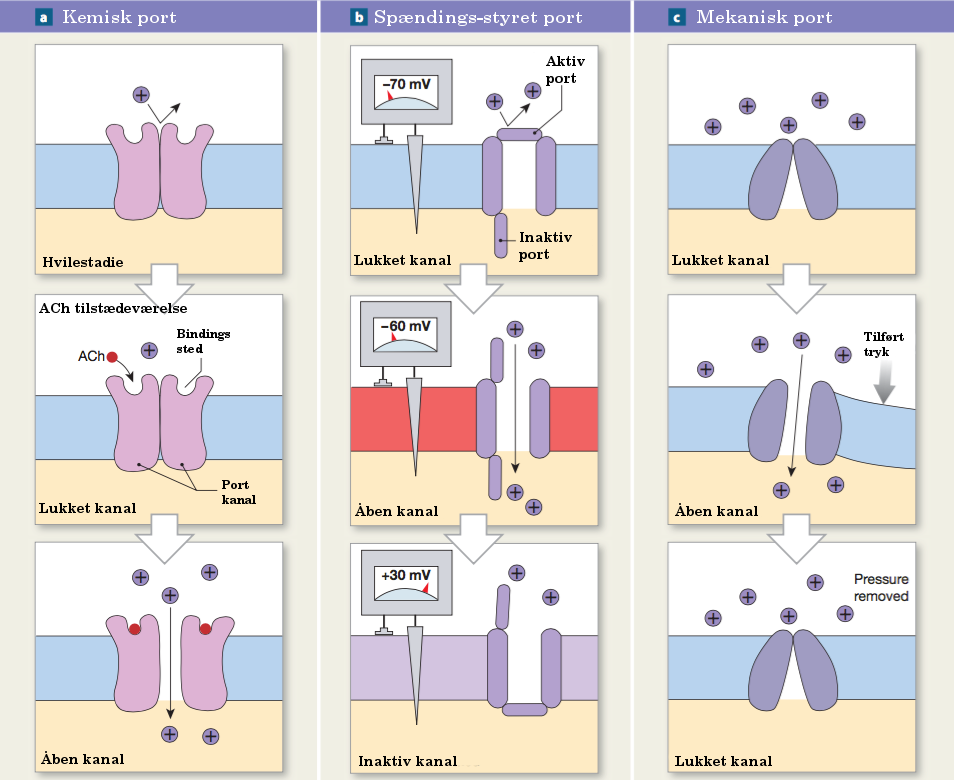
\includegraphics[width=0.5\textwidth]{figures/neuronport}
%	\end{center}
%		\caption{a) Kemisk styret ionkanal der responderer på en kemisk binding b) Spændings styret ionkanal. Ionkanalen åbner ved ændring det transmembrane potentiale c) Mekanisk styret ionkanaler, som ved åbner ved mekanisk stimuli.   \citep{Martini}}
%		\label{neuronport}
%		\centering
%\end{figure}
%%Figuren er fra side 390 i Martini %% OBS, noget ift. frienerveender, og omkring transmembranpot.

%Termoreceptorer er ikke illustreret på figur \ref{neuronport}, men fungerer ved at proteinerne som portene består af, åbner sig ved bestemte temperaturer og derved lader natrium og kalium passere igennem \citep{kimball}. 
%Når en eller flere af disse typer porte åbner strømmer natrium ind i neuronet, mens kalium strømmer ud, og neuronets membranpotentiale stiger. Et gradientpotentiale opbygges og hvis dette er tilstrækkelig højt opnås neuronets tærskelværdi, og et aktionspotentiale sendes afsted. Dette potentiale når til en synapsespalte mellem to neuroner, hvor potentialet overføres ved frigivelse af kemiske transmitterstoffer, som acetylcholin (ACh). Modtagerneuronet har ACh recptorer som igangsætter opbygningen af et gradientpotentiale, så impulsen kan fortsætte. \\
%Impulsen fortsætter ad neuronerne til en dorsal ganglion, hvor flere neuroner samles inden de ledes ind i henholdsvis rygmarvens spinothalamiske tragt eller den posteriore søjle, afhængig af om de bringer information om upræcis berøring, tryk, temperatur og smerte, eller præcis berøring, vibration og proprioception. \citep{Martini}

%sendes til centralnervesystemet (CNS), hvor det først når rygmarven og lidt senere hjernen. Her skelnes der mellem smerte sensation og perception. Smertesensation er information om smerte, som nerverne i hånden der registrere den skadelige temperatur. Smerte perceptionen sker først når nervesignalet når op til hjernen og denne modtager signalet og opfatter det som smerte. Sensationen af smerte kan i rygsøjlen aktivere en refleks der får musklerne i armen til at trække hånden væk fra varmen, inden hjernen når at registrere og opfatte den egentlige smerte. \citep{Martini} Denne form for smerte er kategoriseret som akut-nødvendig smerte, da det hjælper kroppen med at undgå skader.

%Modsat akut-nødvendig smerte findes unødvendig smerte. Denne smerte kaldes også kronisk smerte, da den oftest er længerevarende, ved at have været konstant i mindst tre måneder \citep{Giangregorio1997}. 

% kilde der siger at nociceptisk smerter både er akut og kronisk: http://www.slideshare.net/ssakpi/molecular-mechanisms-of-pain-part-1
% kilde der siger at akut og kronisk smerte er to helt forskellige ting, hvor nociceptisk og neuropatisk begger er under kronisk: http://www.denalihealthcaremi.com/tag/classification-of-pain/
% kilde som siger at smerte kan opdeles efter hvordan det bestemmes: udfra længde af smerten eller udfra smertens natur (oprindelse)
% hvis man skære en nerve over, burde smerten kunne kategoriseres som akut, men idet det er en skade på en nerve er det neuropatisk og derfor kronisk smerte?


